\documentclass{standalone}
\usepackage{tikz}
\usetikzlibrary{patterns, positioning}

\begin{document}
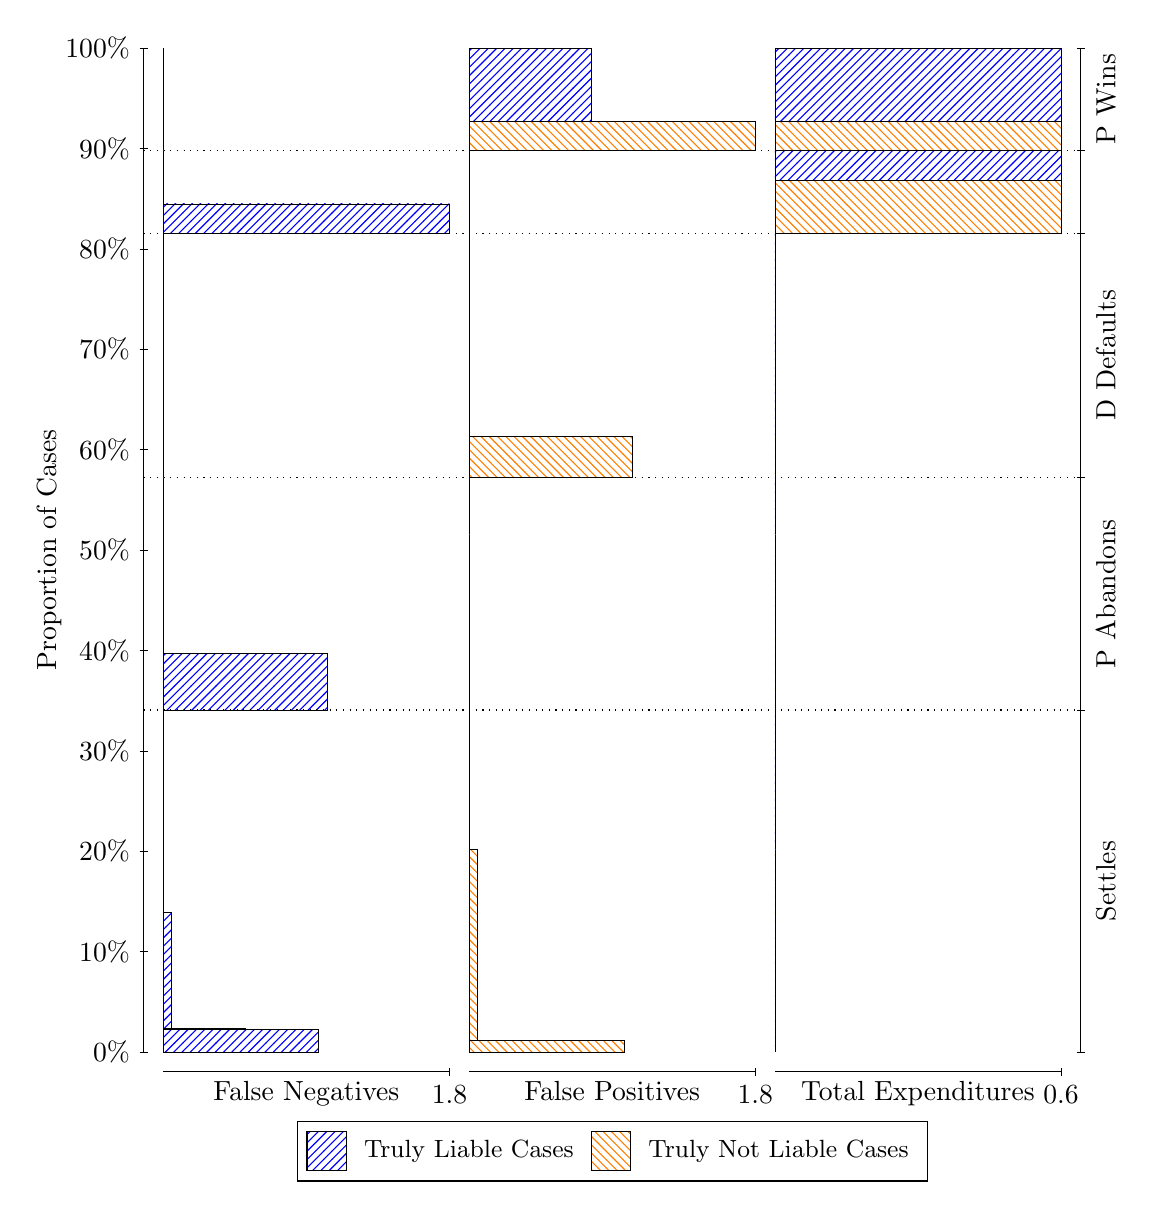
\begin{tikzpicture}
\draw[black, very thin] (1.5,1.75) -- (1.5,14.5);
\node[rotate=90, anchor=center] at (0.3, 8.125) {Proportion of Cases};
\draw[black, very thin] (1.45,1.75) -- (1.55,1.75);
\node[anchor=east] at (1.45, 1.75) {0\%};
\draw[black, very thin] (1.45,3.025) -- (1.55,3.025);
\node[anchor=east] at (1.45, 3.025) {10\%};
\draw[black, very thin] (1.45,4.3) -- (1.55,4.3);
\node[anchor=east] at (1.45, 4.3) {20\%};
\draw[black, very thin] (1.45,5.575) -- (1.55,5.575);
\node[anchor=east] at (1.45, 5.575) {30\%};
\draw[black, very thin] (1.45,6.85) -- (1.55,6.85);
\node[anchor=east] at (1.45, 6.85) {40\%};
\draw[black, very thin] (1.45,8.125) -- (1.55,8.125);
\node[anchor=east] at (1.45, 8.125) {50\%};
\draw[black, very thin] (1.45,9.4) -- (1.55,9.4);
\node[anchor=east] at (1.45, 9.4) {60\%};
\draw[black, very thin] (1.45,10.675) -- (1.55,10.675);
\node[anchor=east] at (1.45, 10.675) {70\%};
\draw[black, very thin] (1.45,11.95) -- (1.55,11.95);
\node[anchor=east] at (1.45, 11.95) {80\%};
\draw[black, very thin] (1.45,13.225) -- (1.55,13.225);
\node[anchor=east] at (1.45, 13.225) {90\%};
\draw[black, very thin] (1.45,14.5) -- (1.55,14.5);
\node[anchor=east] at (1.45, 14.5) {100\%};

\draw[black, very thin] (13.4,1.75) -- (13.4,14.5);
\draw[black, very thin] (13.35,1.75) -- (13.45,1.75);
\node[anchor=west] at (13.35, 1.75) {};
\draw[black, very thin] (13.35,6.093) -- (13.45,6.093);
\node[anchor=west] at (13.35, 6.093) {};
\draw[black, very thin] (13.35,9.0469) -- (13.45,9.0469);
\node[anchor=west] at (13.35, 9.0469) {};
\draw[black, very thin] (13.35,12.145) -- (13.45,12.145);
\node[anchor=west] at (13.35, 12.145) {};
\draw[black, very thin] (13.35,13.197) -- (13.45,13.197);
\node[anchor=west] at (13.35, 13.197) {};
\draw[black, very thin] (13.35,14.5) -- (13.45,14.5);
\node[anchor=west] at (13.35, 14.5) {};

\draw[black, very thin, pattern color=blue, pattern=north east lines] (1.75,1.75) rectangle (3.7224,2.0407);
\draw[black, very thin, pattern color=blue, pattern=north east lines] (1.75,2.0407) rectangle (2.7881,2.0485);
\draw[black, very thin, pattern color=blue, pattern=north east lines] (1.75,2.0485) rectangle (1.8538,3.524);
\draw[black, very thin, pattern color=orange, pattern=north west lines] (1.75,3.524) rectangle (1.75,6.093);
\draw[black, very thin, pattern color=blue, pattern=north east lines] (1.75,6.093) rectangle (3.8262,6.8164);
\draw[black, very thin, pattern color=orange, pattern=north west lines] (1.75,6.8164) rectangle (1.75,9.0469);
\draw[black, very thin, pattern color=orange, pattern=north west lines] (1.75,9.0469) rectangle (1.75,9.5705);
\draw[black, very thin, pattern color=blue, pattern=north east lines] (1.75,9.5705) rectangle (1.75,12.145);
\draw[black, very thin, pattern color=blue, pattern=north east lines] (1.75,12.145) rectangle (5.3833,12.52);
\draw[black, very thin, pattern color=orange, pattern=north west lines] (1.75,12.52) rectangle (1.75,13.197);
\draw[black, very thin, pattern color=orange, pattern=north west lines] (1.75,13.197) rectangle (1.75,13.572);
\draw[black, very thin, pattern color=blue, pattern=north east lines] (1.75,13.572) rectangle (1.75,14.5);
\draw[black, very thin, pattern color=orange, pattern=north west lines] (5.6333,1.75) rectangle (7.6057,1.8954);
\draw[black, very thin, pattern color=orange, pattern=north west lines] (5.6333,1.8954) rectangle (6.6714,1.9016);
\draw[black, very thin, pattern color=orange, pattern=north west lines] (5.6333,1.9016) rectangle (5.7371,4.319);
\draw[black, very thin, pattern color=blue, pattern=north east lines] (5.6333,4.319) rectangle (5.6333,6.093);
\draw[black, very thin, pattern color=orange, pattern=north west lines] (5.6333,6.093) rectangle (5.6333,8.3235);
\draw[black, very thin, pattern color=blue, pattern=north east lines] (5.6333,8.3235) rectangle (5.6333,9.0469);
\draw[black, very thin, pattern color=orange, pattern=north west lines] (5.6333,9.0469) rectangle (7.7095,9.5705);
\draw[black, very thin, pattern color=blue, pattern=north east lines] (5.6333,9.5705) rectangle (5.6333,12.145);
\draw[black, very thin, pattern color=orange, pattern=north west lines] (5.6333,12.145) rectangle (5.6333,12.822);
\draw[black, very thin, pattern color=blue, pattern=north east lines] (5.6333,12.822) rectangle (5.6333,13.197);
\draw[black, very thin, pattern color=orange, pattern=north west lines] (5.6333,13.197) rectangle (9.2667,13.572);
\draw[black, very thin, pattern color=blue, pattern=north east lines] (5.6333,13.572) rectangle (7.1905,14.5);
\draw[black, very thin, pattern color=orange, pattern=north west lines] (9.5167,1.75) rectangle (9.5167,4.319);
\draw[black, very thin, pattern color=blue, pattern=north east lines] (9.5167,4.319) rectangle (9.5167,6.093);
\draw[black, very thin, pattern color=orange, pattern=north west lines] (9.5167,6.093) rectangle (9.5167,8.3235);
\draw[black, very thin, pattern color=blue, pattern=north east lines] (9.5167,8.3235) rectangle (9.5167,9.0469);
\draw[black, very thin, pattern color=orange, pattern=north west lines] (9.5167,9.0469) rectangle (9.5167,9.5705);
\draw[black, very thin, pattern color=blue, pattern=north east lines] (9.5167,9.5705) rectangle (9.5167,12.145);
\draw[black, very thin, pattern color=orange, pattern=north west lines] (9.5167,12.145) rectangle (13.15,12.822);
\draw[black, very thin, pattern color=blue, pattern=north east lines] (9.5167,12.822) rectangle (13.15,13.197);
\draw[black, very thin, pattern color=orange, pattern=north west lines] (9.5167,13.197) rectangle (13.15,13.572);
\draw[black, very thin, pattern color=blue, pattern=north east lines] (9.5167,13.572) rectangle (13.15,14.5);
\draw[black, dotted] (1.5,6.093) -- (13.4,6.093);
\draw[black, dotted] (1.5,9.0469) -- (13.4,9.0469);
\draw[black, dotted] (1.5,12.145) -- (13.4,12.145);
\draw[black, dotted] (1.5,13.197) -- (13.4,13.197);
\draw[black, very thin] (1.75,1.5) -- (5.3833,1.5);
\node[anchor=north] at (3.5667, 1.5) {False Negatives};
\draw[black, very thin] (5.3833,1.45) -- (5.3833,1.55);
\node[anchor=north] at (5.3833, 1.45) {1.8};

\draw[black, very thin] (5.6333,1.5) -- (9.2667,1.5);
\node[anchor=north] at (7.45, 1.5) {False Positives};
\draw[black, very thin] (9.2667,1.45) -- (9.2667,1.55);
\node[anchor=north] at (9.2667, 1.45) {1.8};

\draw[black, very thin] (9.5167,1.5) -- (13.15,1.5);
\node[anchor=north] at (11.333, 1.5) {Total Expenditures};
\draw[black, very thin] (13.15,1.45) -- (13.15,1.55);
\node[anchor=north] at (13.15, 1.45) {0.6};

\node[black, centered, rotate=90] at (13.72, 3.9215) {Settles};
\node[black, centered, rotate=90] at (13.72, 7.57) {P Abandons};
\node[black, centered, rotate=90] at (13.72, 10.596) {D Defaults};

\node[black, centered, rotate=90] at (13.72, 13.849) {P Wins};

\draw (7.449999999999999,1.5) node[draw=none] (baseCoordinate) {};
\begin{scope}[align=center]
        \matrix[scale=0.5, draw=black, below=0.5cm of baseCoordinate, nodes={draw}, column sep=0.1cm]{
            \node[rectangle, draw, minimum width=0.5cm, minimum height=0.5cm, pattern=north east lines, pattern color=blue] {}; &
            \node[draw=none, font=\small] (B) {Truly Liable Cases}; &
            \node[rectangle, draw, minimum width=0.5cm, minimum height=0.5cm, pattern=north west lines, pattern color=orange] {}; &
            \node[draw=none, font=\small] (B) {Truly Not Liable Cases}; \\
            };
\end{scope}

\end{tikzpicture}
\end{document}